\section{Modern mixed-integer linear programming solvers}

In this chapter, we will discuss some of the numerous features that are shared by most professional-grade implementation of mixed-integer programming (MIP) solver. As it will become clear, MIP solvers are formed by an intricate collection of techniques that have been developed through the last few decades. The continuous improvement and development of new such techniques have enabled performance improvements beyond purely hardware performance progress. In fact, this is a very lively and exciting research area, with new features being proposed and incorporated in these solvers with frequent new releases of these tools.

The main difference between MIP solver implementations is which ``tricks'' and techniques they have implemented. In some cases, these are not disclosed in full detail, since the high-performing solvers are commercial products subject to trade secrets. Luckily, some open-source (such as CBC and HiGHS) and free-to-use alternatives (such as SCIP) have been made available, but they are not up to par with commercial implementations in terms of performance as yet.

We will focus on describing the most important techniques forming a professional-grade MIP solver implementation. Most MIP solvers allow for significant tuning and on-off toggling of these techniques. Therefore, knowing the most important techniques and how they work can be beneficial in configuring MIP solvers to your own needs.

Most MIP solvers implement a method that is called \emph{branch-and-cut} which consists of a combination of the linear-programming (LP)-based branch-and-bound method (as described in Chapter \ref{chapter_9}) and a cutting-plane method (as described in Chapter \ref{chapter_10}) that is employed at the root note (or the first subproblem LP relaxation) and possibly at later nodes as well. Figure \ref{p1c11:fig:MIP_solver_flowchart} illustrates the typical flowchart of a MIP solver algorithm.

\begin{figure}
	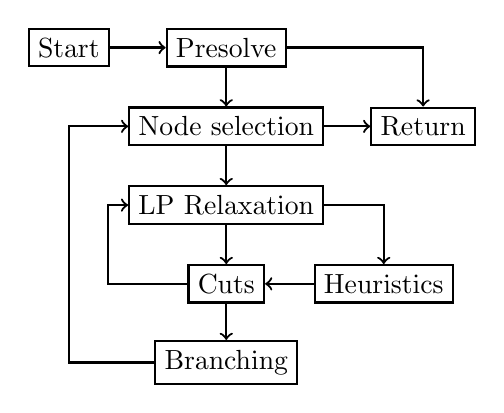
\begin{tikzpicture}[scale=1, node/.style={draw, thick}]
		\node[node] (Start) at (0,6) {Start};
		\node[node] (Presolve) at (2,6) {Presolve};
		\node[node] (Return) at (4.5,5) {Return};
		\node[node] (Node selection) at (2,5) {Node selection};
		\node[node] (LP relaxation) at (2,4) {LP Relaxation};
		\node[node] (Cuts) at (2,3) {Cuts};
		\node[node] (Branching) at (2,2) {Branching};
		\node[node] (Heuristics) at (4,3) {Heuristics};
		% Arrows
		\draw[thick, ->] (Start) --(Presolve);
		\draw[thick, ->] (Presolve) -- (Node selection);
		\draw[thick, ->] (Presolve) -- (4.5,6) -- (Return);
		\draw[thick, ->] (Node selection) -- (LP relaxation);
		\draw[thick, ->] (Node selection) -- (Return);
		\draw[thick, ->] (LP relaxation) -- (Cuts);
		\draw[thick, ->] (LP relaxation) -- (4,4) -- (Heuristics);
		\draw[thick, ->] (Cuts) -- (Branching);
		\draw[thick, ->] (Heuristics) -- (Cuts);
		\draw[thick, ->] (Branching) -- (0,2) -- (0,5) --(Node selection);
		\draw[thick, ->] (Cuts) -- (0.5,3) -- (0.5,4) -- (LP relaxation);
	\end{tikzpicture} 
	\caption{The flowchart of a typical MIP solver. The nodes represent phases of the algorithm} \label{p1c11:fig:MIP_solver_flowchart}
\end{figure}

The first phase consists of a preprocessing phase called \emph{presolve}. In that, the problem formulation is analysed to check whether redundant constraints or loose variables can be trivially removed. In addition, more sophisticated techniques can be employed to try to infer the optimal value of some variables via logic or to tighten their bounds. For simple enough problems, the presolve might be capable of returning an optimal solution or a certificate that the problem is infeasible or unbounded.

Then, the main solution loop starts, similarly to what we have described in Chapter \ref{chapter_9} when discussing the branch-and-bound method. A node selection method is employed and the LP relaxation is solved. Then, branching is applied and the process continues until an optimal solution has been found. 

The main difference however relates to the extra \emph{Cuts} and \emph{Heuristics} phases. Together with the \emph{presolve}, this is likely the phases that most differ between implementations of MIP solvers. The cut phase consists of the employment of a cutting-plane method onto the current LP relaxation with the aim of either obtaining an integer solution (and thus pruning the branch by optimality) or strengthening the formulation of the LP relaxation, as discussed in Chapter \ref{chapter_10}. Each solver will have their own family of cuts that is used in this phase, and typically a collection of them are used simultaneously. The heuristics phase is used in combination to try to obtain primal feasible solutions from the LP relaxations (possibly augmented by cuts) so primal bounds (integer and feasible solution values) can be obtained and broadcasted to the whole search tree, hopefully fostering pruning by bound. 

In what follows, we will discuss the main techniques in each of these phases. 


\section{Presolving methods}

Presolving (or preprocessing) methods are methods typically employed before the start of the branch-and-cut method. These methods have three main goals: (i) reducing the problem size by fixing variables and eliminating constraints; (ii) strengthening the LP relaxation by identifying bounds and coefficients that can be tightened; and (iii) exploiting integrality to improve formulation and identify problem structures (e.g., knapsack or assignment structures)


\subsubsection{Detecting infeasibility and redundancy}

Many techniques used in the preprocessing phase relies on the notion of constraint activity. Consider the constraint $a^\top x \leq b$, with $x \in \reals^n$ as a decision variable vector, $l \leq x \leq u$, $b \in \reals$, where $(a,b,l,u)$ are given. We say that the \emph{minimum activity} of the constraint is given by
%
\begin{equation*}
	\alpha_{\text{min}} = \min\braces{a^\top x : l \leq x \leq u} = \sum_{j : a_j > 0}a_jl_j + \sum_{j : a_j < 0}a_j u_j.	
\end{equation*}
%
Analogously, the \emph{maximum activity} of a constraint is given by 
%
\begin{equation*}
	\alpha_{\text{max}} \hspace{-2pt} = \max\braces{a^\top x : l \leq x \leq u} = \sum_{j : a_j > 0}a_ju_j + \sum_{j : a_j < 0}a_jl_j
\end{equation*}

Notice that the constraint activity is simply capturing what is the minimum and maximum (respectively) values the left-hand side of $a^\top x \leq b$ could assume. This constraint activity can be used in number of ways. For example, if there is a constraint for which $\alpha_{\text{min}} > b$, then the problem is trivially \emph{infeasible}. On the other hand, if one observes that $\alpha_{\text{max}} \leq b$ for a given constraint, then the constraint can be safely removed since it is guaranteed to be redundant.


\subsubsection{Bound tightening}

Another important presolving method is bound tightening, which, as the name suggests, tries to tighten lower and upper bounds of variables, thus strengthening the LP relaxation formulation. There are alternative ways that this can be done, and they typically trade off how much tightening can be observed and how much computational effort they require. 

One simple way of employing bound tightening is by noticing the following. Assume, for simplicity, that $a_j > 0$ $\forall j \in J$. Then, we have that
%
\begin{equation*}
	\alpha_{\text{min}} = \sum_{j \in J}a_jl_j = a^\top l \le a^\top x \le b,
\end{equation*}
%
where $l \in \reals^{|J|}$.
From the second inequality, we obtain 
%
\begin{align*}
    a_jx_j \le b - a^\top x + a_jx_j.
\end{align*}
%
Let $a^\top = (\overline{a}, a_j)^\top$, $x = (\overline{x}, x_j)$ and $l = (\overline{l}, l_j)$, then we have $\alpha_{\text{min}} = a^\top l = \overline{a}^\top \overline{l} + a_j l_j$ and $a^\top x = \overline{a}^\top \overline{x} + a_j x_j$. By the definition of \emph{minimum activity}, we know that $\overline{\alpha}_{\text{min}} = \overline{a}^\top \overline{l} \le \overline{a}^\top \overline{x}$, which is equivalent to 
%
\begin{align*}
    \alpha_{\text{min}} - a_jl_j \le a^\top x - a_jx_j.
\end{align*}
%
This can be reformulated as 
%
\begin{align*}
    b - a^\top x + a_jx_j \le b - \alpha_{\text{min}} + a_jl_j.
\end{align*}
%
Combining this result with what was obtained from the second inequality, we have that
\begin{equation*}
	 a_jx_j \le b - a^\top x + a_jx_j \le b - \alpha_{\text{min}} + a_jl_j,
\end{equation*}
%
from which we can extract the bound
%
\begin{equation*}
	x_j \leq \frac{b - \alpha_{\text{min}} + a_jl_j}{a_j},
\end{equation*}
%
that is, an upper bound for $x_j$. The procedure can be analogously adapted to obtain a lower bound as well. Furthermore, rounding can be employed in the presence of integer variables. 

Another common bound tightening technique consists of solving a linear programming subproblem for each variable variable $x_j$, $j =1, \dots, n$. Let
%
\begin{equation*}
	IP : \mini \braces{c^\top x : x \in X = P \cap \integers^n}		
\end{equation*}
%
where $P$ is a polyhedral set. Then, optimal solution value of the subproblem
%
\begin{equation*}
	LP_{x_j} : \mini \braces{x_j : x \in P}		
\end{equation*}
%
provides a lower bound for $x_j$ that considers all possible constraints at once. Analogously, solving $LP_{x_j}$ as a maximisation problem yields an upper bound. Though this can be done somewhat efficiently, this clearly has steeper computational requirements. 

\subsubsection{Coefficient tightening}

Differently from bound tightening, coefficient tightening techniques aim at improving the strength of existing constraints. The simplest form consists of the following. Let $a_j > 0$, $x_j \in \braces{0,1}$, such that $\alpha_{\text{max}} - a_j < b$. If such coefficients are identified, then the constraint 
%
\begin{equation*}
	a_jx_j + \sum_{j' : j' \neq j} a_{j'}x_{j'}\leq b
\end{equation*}
%
can be modified to become
%
\begin{equation*}
	(\alpha_{\text{max}} - b)x_j + \sum_{j' : j' \neq j} a_{j'}x_{j'} \leq (\alpha_{\text{max}} - a_j).
\end{equation*}
%
Notice that the modified constraint is valid for the original integer set, while dominating the original constraint (cf. Definition \ref{p1c10:def:dominance} since, on the lefthand side, we have that $\alpha_{\text{max}} - b < a_j$ and on the righthand side wee have $\alpha_{\text{max}} - a_j < b$).


\subsubsection{Other methods}

There are a wide range of methods employed as preprocessing, and they vary greatly among different solvers, and even different modelling languages. Thus, compiling an exhaustive list is no trivial feat. Some other common methods that are employed include:
\begin{itemize}
	\item {\bf Merge of parallel rows and columns}: methods implemented to identify pairs of rows (constraints) and columns (variables) with constant proportionality coefficient (i.e., are linearly dependent) and merge them into a single entity, thus reducing the size of the model.
	\item {\bf Domination tests between constraints}: heuristics that test whether domination between selected constraints can be asserted so that some constraints can be deemed redundant and removed. 
	\item {\bf Clique merging}: a clique is a subset of vertices of graph that are fully connected. Assume that $x_j \in \braces{0,1}$ for $j \in \braces{1,2,3}$ and that the three constraints hold:
	\begin{align*}
		& x_1 + x_2 \le 1 \\
		& x_1 + x_3 \le 1 \\
		& x_2 + x_3 \le 1.
	\end{align*}
	Then, one can think of these constraints forming a clique between the imaginary nodes 1, 2, and 3, which renders the clique cut $x_1 + x_2 + x_3 \le 1$. Many other ideas using this graph representation of implication constraints, known as \emph{conflict graphs} are implemented in presolvers.
	\item {\bf Greatest common denominator (GCD) reduction}: We can use the GCD of the coefficients $a = [a_1, \dots, a_n]$ to generate or tighten inequalities. Let $\text{{\bf gcd}}(a)$ be the GCD of all coefficients $a_j$ in $a$. Then we can generate the valid inequality
	\begin{equation*}
		\sum_{j=1}^n\frac{a_j}{\text{{\bf gcd}}(a)} x_j\leq \left\lfloor\frac{b}{\text{{\bf gcd}}(a)}\right \rfloor.
	\end{equation*}
\end{itemize}

 
Some final remarks are worth making. Most solvers might, at some point in the process of solving the MIP refer to something called \emph{restart}, which consists of reapplying some or all of the techniques associated with the preprocessing phase after a few iterations of the branch-and-cut process. This can be beneficial since in the solution process new constraints are generated (cuts) which might lead to new opportunities for reducing the problem or further tightening bounds.

In addition, conflict graphs can contain information that can be exploited in a new round of preprocessing and transmitted across all search tree, a process known as propagation. Conflict graphs and propagation are techniques originally devised for constraint programming and satisfiability (SAT) problems, but have made considerable inroads in MIP solvers as well.


\section{Cut generation}

One major component of MIP solvers is its cut generation procedures. In practice, MIP solvers implement what is called \emph{branch-and-cut}, which is a method formed by the amalgamation of branch-and-bound (as we seen in Chapter \ref{chapter_9}) and cutting-plane methods (Chapter \ref{chapter_10}). In fact, the combination of both methods is arguably the most important methodological development that ultimately rendered MIP solvers reliable to be used in practice in many applications. 

There is an interesting symbiotic relationship emerging from the combination of the two methods. In general, cutting planes are useful in tightening the existing formulation but often fail in being able to generate all the cuts required to expose an integer optimal solution. On the other hand, branch-and-bound might require considerable computational efforts to adequately expose the integer optimal solutions of all subproblems, but is guaranteed to converge in finite time (even if this time is not feasible in a practical sense). Thus, the combination of both allows for a method that is far more likely to terminate within reasonable computation time.

However, some care must be considered when generating cuts in branch-and-cut settings, since it can quickly increase the dimension of the subproblems, which would lead to amplified consequences to the performance of the branch-and-bound part. This is mitigated with a feature called \emph{cut pool}, which consists of a way to make sure that only selected cuts, e.g., cuts that are violated by the solution of the relaxation, are considered in the subproblem. Such cuts are chosen using what is referred to as cut selection routines.

Furthermore, most professional-grade solvers allow for the definition of user cuts, which are user-defined cuts that are strongly problem specific, but give strong customisation powers to advanced users. As it turns out, the types of cuts available is one of the main differentiators between solvers and the search for cuts that are both efficient and generic is an active research and development direction.

The most common types of cuts utilised include fractional (or Gomory) cuts, of the form
%
\begin{equation*}
	\sum_{j \in I_N} f_{ij}x_j \geq f_{i0}, \text{ where } f_{ij} = \overline{a}_{ij} - \floor{\overline{a}_{ij}}
\end{equation*}
%
and Chv\'atal-Gomory cuts for pure integer constraints, which are dependent on the heuristic or process used to define the values of the multipliers $u$ in
% 
\begin{equation*}
	\sum_{j=1}^n  \floor{uA_j}x_j \leq \floor{ub}.
\end{equation*} 
%
For example, zero-half cuts (with $u \in [0,1/2]$) and mod-k cuts ($u \in \braces{0, 1/k, \dots, (k-1)/k}$) are available in most solvers. Other cuts such as knapsack (or cover) inequalities, mixed-integer rounding, clique as also common and, although it can be shown to be related to the Chv\'atal-Gomory procedure, are generated by means of heuristics (normally referring to a cut generation procedure).


\subsection{Cut management: generation, selection and discarding}

With the numerous possibilities of cuts to be generated, it becomes clear that one must be mindful of the total of cuts generated and its associated trade-offs. These trade-offs are managed taking into account which cuts to generate and which cuts to select from the cut pool to be added to the problem. In particular, in case of the generation and selection of cuts, this can often be influenced by users, by selecting how ``aggressively'' cuts are generated.

For example, although dual simplex is perfectly suited for resolving the linear programming (LP) relaxation after the addition of cuts, if multiple cuts are added at once, it might mean that resolving the LP relaxation from the previous dual optimal basis is not much more beneficial than resolving the LP relaxation from scratch. Moreover, adding cuts increases the size of the basis in the problem, which in turn increases the size of the basic matrix $B$ and its inverse $B^-1$, thus gradually increasing the time per iteration of the method. Lastly, some cuts might require the solution of a demanding separation problem, e.g., lifted cover inequalities. Although these can provide considerable improvements to the formulation, the computational effort required for generating them might dampen the performance improvement they incur.

Selecting which cuts would be the most efficient is not an easy task. Ideally, we would like to chose the minimal number of cuts that has the most impact in terms of improving the LP relaxation. Cleary, we can only try to achieve this via proxies. Solvers normally associate a scoring to each cut taking into account a collection of criteria and these scores are then used in the process of selecting the cuts (their cut selection routines), e.g., selecting a fraction of the top scorer cuts or discarding those that the score is below a certain threshold.

One criteria for trivially discarding cuts is numerical stability. Cuts with too large or too small coefficients are prone to cause numerical issues due to the matrix decomposition methods employed. Therefore, these can be easily disregarded in the selection process. 

An important proxy for efficiency is the notion of \emph{depth} of the cut. That is, a cut can have its depth measured by the distance between the hyperplane that forms the cut and the solution of the LP relaxation. The larger this distance, the ``deeper'' the cut is cutting through the LP relaxation, which could potentially mean that the cut is more efficient. 

Another important proxy is \emph{orthogonality}. Cuts that are pairwise orthogonal with other cuts are likely to be more effective. This is easy to see if you think of the extreme case of zero orthogonality, or the cuts being parallel, clearly meaning that one of the cuts is dominated by the other. Orthogonality can also be measured against the objective function, in which case we are interested in cuts that are almost parallel (but not exactly, as this would lead to numerical issues) to the objective function since those are more likely to cause improvement in the dual bound (LP relaxation optimal) value.


\section{Variable selection: branching strategy}

As we discussed in Chapter \ref{chapter_9}, some decisions in terms of selecting variables to branch and subproblems to solve can have a great impact in the total number of subproblems solved in a branch-and-bound method. Variable selection is still a topic under intensive research, with newer ideas only recently being made available in the main solvers. 

Variable selection, commonly referred to as branching strategies in most MIP solver implementations, refer to the decision of which of the currently fractional variables should be chosen to generate subproblems. There are basic three main methods most commonly used, which we discuss next. Furthermore, most MIP solvers allow for the user to set priority weights to the variables, which defines priority orders for variable selection. These can be useful for example when the user knows that the problem possess a dependence structure between variables (e.g., location and allocation variables, where allocation can only happen if the location decision is made) that the solver cannot infer automatically. 


\subsubsection{Maximum infeasibility}

The first branching strategy, sometimes called \emph{maximum infeasibility}, consists of choosing the variable with the fractional part as close to 0.5 as possible, or, more precisely select the variables $j \in \braces{1, \dots, n}$ as
%
\begin{equation*}
	\arg\max_{j \in \braces{1,\dots,n}} \min\braces{f_j, 1 - f_j} 	
\end{equation*}
%
where $f_j = x_j - \lfloor x_j \rfloor$. This in effect is trying to reduce as most as possible the infeasibility of the LP relaxation solution, which in turn would more quickly lead to a feasible (i.e., integer) solution. A analogous form, called \emph{minimum infeasibility} is often available, and as the name suggests, focus on selecting the variables that are closer to be integer valued.

\subsubsection{Strong branching}

Strong branching can be understood as an explicit look-ahead strategy. That is, to decide which variable to branch on, the method performs branching on all possible variables, and choose that provides the best improvement on the dual (LP relaxation) bound. Specifically, for each fractional variable $x_j$, we can solve the LP relaxations corresponding to branching options $x_j \leq \lfloor x^\text{LP} \rfloor$ and $x_j \geq \lceil x^\text{LP} \rceil$ to obtain LP relaxation objective values $Z_j^D$ and $Z_j^U$. We then choose the fractional variable $x_j$ that leads to subproblems with the best LP relaxation objective values, defined as 
%
\begin{equation*}
	\arg\max_{j \in \braces{1,\dots,n}} \min\braces{Z_j^D, Z_j^U}, 	
\end{equation*}
% 
assuming a minimization problem. Strong branching thus compares the worse LP relaxation bound for each fractional $x_j$ and picks the fractional variable for which this value is the best. 

As you might suspect, there is a trade-off related to the observed reduction in the number of nodes explored, given by the more prominent improvement of the dual bound, and how computationally intensive is the method. There are however ideas that can exploit this trade off more efficiently. First, the solution of the subproblems might yield information related to infeasibility and pruning by limit, which can be used in favour of the method. 

Another idea is to limit the number of simplex iterations performed when solving the subproblems associated with each branching option. This allows for using approximate solution of the subproblems and potential savings in computational efforts. Some solvers offer a parameter that allow the user to set this iteration limit value.


\subsubsection{Pseudo-cost branching}

Pseudo-cost branching relies on the idea of using past information from the search process to estimate gains from branching on a specific variable. Because of this reliance on past information, the method tends to be more reliable later in the search tree, where more information has been accumulated on the impact of choosing a variable for branching.

These improvement estimates are the so called \emph{pseudo-costs}, which compile an estimate on much the dual (LP relaxation) bound has improved per fractional unit of the variable that has been reduced. More specifically, let 
%
\begin{equation} \label{p1c11:eq:fractionals}
	f^{-}_j = x^{\text{LP}}_j - \lfloor x^{\text{LP}}_j \rfloor \text{ and } f^{+}_j = \lceil x^{\text{LP}}_j \rceil - x^{\text{LP}}_j.	
\end{equation}
%
Then, we can define the quantities $\Psi^-_j$ and $\Psi^+_j$ to be the average improvement in the dual bound observed per fractional unit reduced and increased, respectively, whenever the variable $x_j$ has been selected for branching, i.e, for each branching direction. Notice that this requires that several subproblems to be solved for a reliable estimate to be available.

Then, we can define the quantities
%
\begin{equation} \label{p1c11:eq:improvement_estimates}
	\Delta^-_j = f^-_j \Psi^-_j \text{ and } \Delta^+_j = f^+_j \Psi^+_j
\end{equation}
%
which represent the estimated change to be observed when selecting the variable $x_j$ for branching, based on the current fractional parts $f^+_j$ and $f^-_j$. In effect, these are considered in a branching score, with the branching variable being selected as, for example, 
%
\begin{equation*}
	j = \argmax_{j=1, \dots, n} \braces{ \alpha \min\braces{\Delta^-_j, \Delta^+_j} + (1-\alpha)\max\braces{\Delta^-_j, \Delta^+_j}}.
\end{equation*}
%
where $\alpha \in [0,1]$. Setting the value of $\alpha$ trades off two aspects. Assume a maximisation problem. Then, setting $\alpha$ closer to zero will slow down \emph{degradation}, which refers to the decrease of the upper bound (notice that the dual bound is decreasing and thus, $\Delta^+$ and $\Delta^-$ are negative). This strategy improves the chances of finding a good feasible solution on the given branch, and, in turn, potentially fostering pruning by bound. In contrast, setting $\alpha$ closer to one increases the rate of decrease (improvement) of the dual bound, which can be helpful for fostering pruning once a good global primal bound is available. Some solvers allow for considering alternatives branching score functions. % XPRESS

As one might suspect, it might take several iterations before reliable estimates $\Psi^+$ and $\Psi^-$ are available. The issue with unreliable pseudo-costs can be alleviated with the use of a hybrid strategy known as \emph{reliability} branching\footnote{Tobias Achterberg, Thorsten Koch, and Alexander Martin (2005), Branching rules revisited, Operations Research Letters}. In that, variables that are deemed unreliable for not having been selected for branching a minimum number of times $\eta \in [4,8]$, have strong branching employed instead.   

 
\subsubsection{GUB branching}
 
Constraints of the form 
%
\begin{equation*}
	\sum_{j = 1}^k x_j = 1	
\end{equation*}
%
are referred to as special ordered sets 1 (or SOS1) which, under the assumption that $x_j \in \braces{0,1}$, $\forall j \in \braces{1,\dots,k}$ implies that only one variable can take value different than zero. Notice you may have SOS1 sets involving continuous variables, which, in turn would require the use of binary variables to be modelled appropriately. 

Branching on these variables might lead to unbalanced branch-and-bound trees. This is because the branch in which $x_j$ is set to a value different than zero, immediately define the other variables to be zero, leading to an early pruning by optimality or infeasibility. In turn, unbalanced trees are undesirable since they preclude the possibility of parallelisation and might lead to issues related to searches that focuses on finding leaf notes quickly.

To remediate this, the idea of using a generalised upper bound is employed, leading to what is referred to as GUB branching (with some authors referring to this as SOS1 branching). A generalised upper bound is an upper bound imposed on the sum of several variables. In GUB branching, branching for binary variables is imposed considering the following rule:
%
\begin{align*}
	&S_1 = S \cap \braces{x : x_{j_i} = 0, \forall i \in \braces{1,\dots,r} } \\
	&S_2 = S \cap \braces{x : x_{j_i} = 0, \forall i \in \braces{r+1,\dots,k} }
\end{align*} 
%
where $r = \argmax_{t \in \braces{1,\dots,k}} \sum_{j=1}^t x_j \leq 0.5$. Notice the upper bounding on the some of the variables, from which the name stems. That is, only a subset of the variables are forced to be zero, while several others are left unconstrained, which favours more balanced search trees. As a final remark, constraint of the form of
%
\begin{equation*}
	\sum_{j = 1}^k x_j \le 1	
\end{equation*}
%
can also benefit of the use of GUB branching, with the term GUB being perhaps better suited in this case. 


\section{Node selection}

We now focus on the strategies associated with selecting the next subproblem to be solved. As we have seen in Chapter \ref{chapter_9}, the order in which the subproblem's LP relaxations are solved can have a major impact on the total number of nodes explored, and, consequently, on the efficiency of the method. The alternative strategies for node selection typically trade off the following
%
\begin{enumerate}
	\item Focus on finding primal feasible solutions earlier, to foster pruning by bound.
	\item Alternatively, focus on improving the dual bound faster, hoping that once an integer solution is found, more pruning by bound is possible.
	\item Increase \emph{ramp-up}, which means increase the number of unsolved nodes in the list of subproblems so that these might be solved in parallel. For that, the nodes must be created, and the faster they are opened, the earlier parallelisation	can benefit the search.
	\item Minimise computational effort by minimising the overhead associated with changing the subproblems to be solved. That means that children nodes are preferred over other nodes, in a way to minimise the changes needed to assemble a starting basis for the dual simplex method.
\end{enumerate}

You might notice that points 1 and 2 are conflicting, since while the former would benefit from a breadth-focused search (that is, having wider trees earlier is preferable than deeper trees) the latter would benefit from searches that dive deeply in the tree searching from leaf nodes. Points 3 and 4 pose exactly the same dilemma: the former benefits from breadth-focusing searches while the latter benefits from depth-focusing searches.

The main strategies for node selection are, to a large extent, ideas to emphasise each or a combination of the above. 

\subsubsection{Depth-first search (DFS) and breadth-first search (BFS)}

A depth-first search focus on diving down in the search tree, prioritising nodes at lower levels. It has the effect of increasing the chances of finding leaves, and potentially primal feasible solutions, earlier. Furthermore, because the problems being successively solved are very similar, with the exception of one additional branching constraint, the dual simplex methods can be efficiently restarted and often fewer iterations are needed to find the optimal of the children subproblem relaxation. On the other hand, as a consequence of the way the search is carried, it is slower in populating the list of subproblems. 

In contrast, breadth-first search gives priorities to nodes higher levels in the tree, ultimately causing a horizontal spread of the search tree. This has as consequence a faster improvement of the dual bound, at the expense of potentially delaying the generation of primal feasible solutions. This also generates more subproblems quickly, fostering diversification (more subproblems and potentially more information to be re-utilised in repeated rounds of preprocessing) and opportunities for parallelisation. 

% TODO: Chp11: improve this description, making it more precise.

\subsubsection{Best bound}

Best bound consists of the strategy of choosing the next node to be that with the best dual (LP relaxation) bound. It leads to a breadth-first search pattern, but with flexibility to allow potentially good nodes that are in deeper levels of the tree to be selected. 

Ultimately, this strategy foster a faster improvement of the dual bound, but with a higher overhead on the set up of the subproblems, since they can be quite different than each other in terms of its constraints. One way to mitigate this overhead is perform \emph{diving} sporadically, which consists of, after choosing a node by best bound, temporarily switching to a DFS search for a few iterations.


\subsubsection{Best estimate or best projection}

Uses a strategy similar to that employing pseudo-costs to choose which variable to branch on. However, instead of focusing on objective function values, it uses estimates of the node progress towards feasibility but relative to its bound degradation. 

To see how this works, assume that the parent node has been solved, and a dual bound $z_D$ is available. Now, using our estimates in \eqref{p1c11:eq:improvement_estimates}, we can calculate an estimate of the potential primal feasible solution value $E$, given by
%
\begin{equation*}
	E = z_D + \sum_{j = 1}^n \min\braces{\Delta^-_j, \Delta^+_j}.	
\end{equation*}
%

The expression $E$ is an estimate of what is the best possible value an integer solution could have if it were to be generated by rounding the LP relaxation solution. These estimates can also take into account the feasibility per se, trying to estimate feasibility probabilities considering known feasible solutions and how fractional the subproblem LP relaxation solution is. 



\section{Primal heuristics}
 
The last element of MIP solvers we must consider are primal heuristics. The term ``primal'' refers to the fact that these are methods geared towards either (i) building primal feasible solutions normally from a solution obtained from a relaxation; or (ii), geared towards improving on previously known primal solutions. The former strategy is often referred to as \emph{constructive} heuristics, while the latter are called \emph{improvement} heuristics. 

The name heuristic refers to the fact that these are methods that are not guided by any optimality certificates per se, but yet by performing local (or nearby, according to a given metric of solution difference) improvements repeatedly.

Primal heuristics play three main important roles in MIP solver algorithms. First, they are employed in the preprocessing phase to verify whether the model can be proved to be feasible, by constructing a primal feasible solution. Second, constructive heuristics are very powerful in generating feasible solutions during the branch-and-bound phase, meaning that it can make primal feasible solutions available \emph{before} they are found at leaf nodes when pruning by optimality (i.e., with integer LP relaxation solution), and therefore fostering early pruning by bound. Lastly, heuristics are a powerful way to obtain reasonably (often considerably) good solutions, which in practical cases, might be sufficient given computational or time limitations and precision requirements.


\subsection{Diving heuristics}

Diving heuristics are used in combination with node selection strategies that search in breadth (instead of depth). In simple terms, it consists of performing a local depth search at the node being considered with no or very little backtracking, with the hope of reusing the subproblem structure while searching for primal feasible solutions. The main difference is that the subproblems are generated in an alternative tree in which branching based on rounding and fixing instead of the standard branching we have seen in Chapter \ref{chapter_9}. 

Once the heuristic terminates, the structure is discarded, but the solution, if found, is kept. Notice that the diving can also be preemptively aborted if it either renders an infeasible subproblem or if it leads to a relaxation with worse bound than a known primal bound from an incumbent solution. Another common termination criteria consists in limiting the total number of LP iterations solving the subproblems or the total number of subproblems solved. 

The most common types of rounding employed in diving heuristics include \emph{fractional diving}, in which the variable selected for rounding is simply that with the smallest fractional component, i.e., $x_j$ is chosen, such that the index $j$ is given by
%
\begin{equation*}
	\argmax_{i=1,\dots,n} \braces{\min\braces{x_i-\lfloor x_i\rfloor, \lceil x_i \rceil - x_i}}.	
\end{equation*}

Another common idea consists of selecting the variables to be rounded by considering a reference solution, which often is an incumbent primal feasible solution. This \emph{guided dive} is then performed by choosing the variable with the smallest fractional value when compared against this reference solution. 

A third idea consists of taking into account the number of \emph{locks} associated with the variable. The locks refer to the number of constraints that are potentially made infeasible by rounding up or down a variable. This potential infeasibility stems from taking into count the coefficient of the variable, the type of constraint constraint and whether rounding it up or down can potentially cause infeasibility. This is referred to as \emph{coefficient diving}.


\subsection{Local searches and large-neighbourhood searches}

Local and large-neighbourhood searches are, contrary to most diving heuristics, improvement heuristics. In these, a reference solution is used to to search for new solutions within its \emph{neighbourhood}. This is simply the idea of limiting any solutions found to share a certain number of elements (for example, have the same values in some components) with the reference solution. We say that a solution is a $k$-neighbour solution if they share $k$ components.

Local search and large-neighbourhood search simply differ in terms of scope; the former allows for only localised change while the latter considers wider possibilities for divergence from the reference solution.

Some of search are seldom used and often turned off by default in professional-grade solvers. They tend to be expensive under a computational standpoint because they require considerable extra work. Most of them are based on fixing and/or relaxing integrality of a number of variables, adding extra constraints and/ or changing objective functions, and resolving which can be considerably onerous. Let us present the most common heuristics found in professional grade solvers. 


\subsubsection{Relaxation-induced neighbourhood search (RINS) and Relaxation-enforced neighbourhood search}

The relaxation-induced neighbourhood search (or RINS) is possibly the most common improvement heuristic available in modern implementations\footnote{Emilie Danna, Edward Rothberg, and Claude Le Pape (2005), Exploring relaxation induced neighborhoods to improve MIP solutions, Mathematical Programming}. The heuristic tries to find solutions that present a balance between proximity of the current LP solution, hoping this would improve the solution quality, and proximity to an incumbent (i.e., best-known primal feasible) solution, emphasising feasibility.

In a nutshell, the method consists of the following. After solving the LP relaxation of a node, suppose we obtain the solution $x^{\text{LP}}$. Also, assume we have at hand an incumbent solution $\overline{x}$. Then, we form an auxiliary MIP problem in which we fix all variables coinciding between $x^{\text{LP}}$ and $\overline{x}$. This can be achieved by including the constraints
	%
	\begin{equation*}
		x_j = \overline{x}_j, \ \forall j \in \braces{1,\dots,n} : \overline{x}_j = x^\text{LP},	
	\end{equation*}
	%
	which,  in effect fix these variables to integer values and remove them from the problem, as they can be converted to parameters (or input data). Notice that this constraints the feasible space to be in the (potentially large) neighbourhood of the incumbent solution. In later iterations, when more of the components of the relaxation solutions $x^{\text{LP}}$ are integer, this becomes a more local search, with less degrees of freedom. Finally, this additional MIP is solved and, in case an optimal solution is found, a new incumbent solution might become available.

In contrast, relaxation-enforced neighbourhood search (or RENS) is a constructive heuristics, which has not yet seem a wider introduction in commercial-grade solvers, though it is available in   CBC and SCIP\footnote{Timo Berthold (2014), RENS: The optimal rounding, Mathematical Programming Computation}.
 
The main differences between RINS and RENS are the fact that no incumbent solution is considered (hence the dropping of the term ``induced'') but rather the LP relaxation solution $x^{\text{LP}}$ fully defines the neighbourhood (explaining the name ``enforced'').
 
Once again, let us assume we obtain the solution $x^{\text{LP}}$. And again, we fix all integer valued variables in $x^{\text{LP}}$, forming a large neighbourhood
%
\begin{equation*}
	x_j = x_j^{\text{LP}}, \ \forall j \in \braces{1,\dots,n} : x_j^{\text{LP}} \in \integers.
\end{equation*}
%

One key difference is how the remaining variables are treated. For those components that are fractional, the following bounds are imposed
%
\begin{equation*}
	\lfloor x_j \rfloor \leq x_j \leq \lceil x_j \rceil, \ \forall j \in \braces{1,\dots,n} : x_j^{\text{LP}} \notin \integers.
\end{equation*}
%
Notice that his in effect makes the neighbourhood considerably smaller around the solution $x^{\text{LP}}$. Then, the MIP subproblem with all these additional constraints is solved and a new incumbent solution may be found. 

 
\subsubsection{Local branching}

The idea of local branching is to allow the search to be performed in a neighbourhood of controlled size, which is achieved by the use of an $L_1$-norm\footnote{Matteo Fischetti and Andrea Lodi (2003), Local branching, Mathematical Programming}. The size of the neighbourhood is controlled by a divergence parameter $\Delta$, which in the case of binary variables, amounts to being the Humming distance between the variable vectors. 

In its most simple form, it can be seen as the following idea. From an incumbent solution $\overline{x}$, one can generate and impose the following neighbourhood inducing constraint
%
\begin{equation*}
	\sum_{j=1}^n | x_j - \overline{x}_j | \leq \Delta
\end{equation*}
%
and then solve the resulting MIP. 

The original use of local branching (as the name suggests) as proposed is to use this constraint directly to form a branching rule in an auxiliary tree search. However, most solvers use it by means of subproblems as  described above.  


  
\subsubsection{Feasibility pump}

Feasibility pump is a constructive heuristic that, contrary to the previous heuristics, has made inroads in most professional-grade solvers and if often employed by default. The focus is exclusively trying to find a first primal feasible solution. The idea consists of, from the LP relaxation solution $x^{\text{LP}}$, performing alternate steps of rounding and solving a projection step, which happens to be a LP problem.

Starting from the $x^{\text{LP}}$, the method starts by simply rounding the components to obtain an integer solution $\overline{x}$. If this rounded solution is feasible, the algorithm terminates. Otherwise, we perform a projection step by replacing the LP relaxation objective function with
	% 
	\begin{equation*}
		f^\text{aux}(x) = \sum_{j = 1}^n |x_j - \overline{x}_j|
	\end{equation*}
	%
	and resolving it. This is called a projection because it is effectively finding a point in the feasible region of the LP relaxation that is the closest to the integer solution $\overline{x}$. This new solution $x^{\text{LP}}$ is once again rounded and the process repeats until a feasible integer solution is found.
	
It is known that feasibility pump can suffer from cycling, that is, repeatedly findingthe same $x^{\text{LP}}$ and $\overline{x}$ solutions. This can be alleviated by performing random perturbations on some of the components of $\overline{x}$.

Feasibility pump is an extremely powerful method and plays a central role in many professional-grade solvers. It is also useful in the context of mixed-integer nonlinear programming models. More recently, variants have been developed\footnote{Timo Berthold, Andrea Lodi, and Domenico Salvagnin (2018), Ten years of feasibility pump, and counting, EURO Journal on Computational Optimization}, taking into account the quality of the projection (i.e., taking into account also the original objective function) and discussing theoretical properties of the methods and its convergence guarantees. 


\pagebreak

\section{Exercises}


\subsection*{Problem 11.1: Preprocessing and primal heuristics}


\begin{itemize}
	\item [(a)] \textit{Tightening bounds and redundant constraints}\\
	
	Consider the LP below,
	\begin{table}[H]
		\centering
		\begin{tabular}{crcrcccc}
			max         &  2$x_1$  & $+$ &   $x_2$  & $-$ &   $x_3$  \vspace{3pt}\\
			s.t.        &  5$x_1$  & $-$ &  2$x_2$  & $+$ &  8$x_3$  & $\leq$ &  15  \vspace{3pt}\\
			&  8$x_1$  & $+$ &  3$x_2$  & $-$ &   $x_3$  & $\leq$ &   9  \vspace{3pt}\\
			&   $x_1$  & $+$ &   $x_2$  & $+$ &   $x_3$  & $\leq$ &   6  \vspace{3pt}\\
			& \multicolumn{3}{c}{0 $\leq x_1 \leq 3$} \vspace{3pt}\\  
			& \multicolumn{3}{c}{0 $\leq x_2 \leq 1$} \vspace{3pt}\\  
			& \multicolumn{3}{c}{$x_3 \geq$ 1},   
		\end{tabular}
	\end{table}

	derive tightened bounds for variables $x_1$ and $x_3$ from the first constraint and eliminate redundant constraints after that. \vspace{10pt}

	\item [(b)] \textit{Primal heuristics (RINS)}\\
	
	Consider the formulation UFL-W:
	\begin{align}
	 \text{(UFL-W)} : \quad &\mini_{x,y} \sum_{j\in N} f_jy_j + \sum_{i\in M}\sum_{j\in N} c_{ij}x_{ij} \label{IP:1}\\
	       &\st\nonumber \\
	       &\quad \sum_{j\in N}x_{ij} = 1, &\forall i \in M,\label{IP:2}\\
	       &\quad \sum_{i\in M}x_{ij} \leq my_j, &\forall  j \in N,\label{IP:3}\\
	       &\quad x_{ij} \geq 0, &\forall i \in M, \forall j \in N,\label{IP:4}\\
	       &\quad y_j \in \{0,1\}, &\forall j\in N,\label{IP:5},
	\end{align}
	
	where $f_j$ is the cost of opening facility $j$, and $c_{ij}$ is the cost of satisfying client $i$'s demand from facility $j$. Consider an instance of the UFL with opening costs $f=(21,16,30,24,11)$ and client costs

	\begin{align*}
	 (c_{ij}) = \left(
		\begin{array}{ccccc}
			6  & 9  & 3 & 4  & 12 \\
			1  & 2  & 4 & 9  & 2  \\
			15 & 2  & 6 & 3  & 18 \\
			9  & 23 & 4 & 8  & 1  \\
			7  & 11 & 2 & 5  & 14 \\
			4  & 3  & 10& 11 & 3
		\end{array}
	 \right)
	\end{align*}

	In the UFL problem, the facility production capacities are assumed to be large, and there is no budget constraint on how many facilities can be built. The problem thus has a feasible solution if at least one facility is opened. We choose an initial feasible solution $\bar{y} = (1,0,0,0,0)$. Try to improve the solution by using relaxation-induced neighbourhood search (RINS) and construct a feasible solution using relaxation-enforced neighbourhood search (RENS). 
\end{itemize}


\subsection*{Problem 11.2: Variable and node selection}
Using Branch-and-Bound, solve the UFL-W problem from the exercises in Chapter 9:
\begin{align}
    \text{(UFL-W)} : \mini_{x,y} & \sum_{j\in N} f_jy_j + \sum_{i\in M}\sum_{j\in N} c_{ij}x_{ij}\\
    \st & \sum_{j\in N}x_{ij} = 1, &\forall i \in M,\\
        & \sum_{i\in M}x_{ij} \leq my_j, &\forall  j \in N,\\
        & x_{ij} \geq 0, &\forall i \in M, \forall j \in N,\\
        & y_j \in \{0,1\}, &\forall j\in N,
\end{align}

with opening costs $f=(4,3,4,4,7)$ and client costs

\begin{equation*}
 (c_{ij}) = \left(
	\begin{array}{ccccc}
		12 & 13 & 6 & 0  & 1 \\
		8  & 4  & 9 & 1  & 2 \\
		2  & 6  & 6 & 0  & 1 \\
		3  & 5  & 2 & 1  & 8 \\
		8  & 0  & 5 & 10 & 8 \\
		2  & 0  & 3 & 4  & 1
	\end{array}
 \right).
\end{equation*}

\begin{itemize}
 \item To obtain a good start for branching, use strong branching at the root node. All following branching variables should be selected using maximum infeasibility.
 \item For node selection, use the best bound selection to minimze the number of evaluated nodes.
\end{itemize}





